% Owners: Hikaru and Kelvin.
% This file controls the order. Edit one experiment file under workload-a/.
\section{Task 2: Optimized Design for Workload A}
\label{sec:optimized-a}

Our strategy followed the measured bottlenecks. We investigated lookup indexes,
data placement and read-only declarations, then targeted T6 after T3 and T4
improved. In parallel, Kelvin evaluated the write path. The main progression was
\expt{a0} to \expt{a102} to \expt{a111} to \expt{a112}: lookup indexes,
join-key colocation, and read-only declarations.

The final design preserves the workload mix, isolation and durability.
Experiment a12 deliberately changes commit durability and is evaluated separately.
Short diagnostics, local tests and full cluster benchmarks are distinguished.

% Hikaru: implementation. Kelvin: full cluster run and analysis.
\subsection{\expt{a102}: Lookup indexes}
\label{sec:a102}
The first experiment added three indexes:
\begin{lstlisting}
CREATE INDEX idx_orders_customer_recent
    ON orders (merchant_id, customer_id, created_at DESC);
CREATE INDEX idx_items_order ON order_items (order_id);
CREATE INDEX idx_inventory_product ON inventory (product_id);
\end{lstlisting}
The orders index follows T3's merchant/customer filtering and recent-order
access pattern. The others support order-item and inventory lookups. This
ordering follows PostgreSQL's guidance on leading equality columns in
multicolumn B-tree indexes \citep{pg-multicolumn}.

Kelvin ran a102 as job 965657. Its throughput was
3.250/3.453/3.543/3.320/3.782/3.398 TPS at 1--64 clients. All measured phases
exited normally and recorded no serialization failures. However, the 16-client
warmup aborted, excluding that case from comparisons requiring both phases
to complete.

Against the preserved baseline, eligible concurrent cases appeared 49--57\%
faster. Against the fresh baseline, differences were only approximately
$-3\%$ to $+6\%$. Different node allocations and single observations prevent
a large overall throughput claim attributable to the indexes.

At one client, T7's mean latency decreased from 51.114 to 13.709\,ms, while
T3 and T4 remained expensive at 2,668.472 and 454.362\,ms. The indexes helped
particular operations but did not remove the dominant distributed-read cost.
\evidence{\expt{a102}, job 965657; preserved a0 job 918524 and fresh a0 job
977740. Source identity was checked against the saved runtime hashes.}

% Hikaru.
\subsection{\expt{a101}: Merchant-based colocation}
Experiment a101 distributed merchant-owned data by \code{merchant_id}.
The motivation was to place data used by merchant-scoped transactions together
and reduce distributed execution, following Citus's tenant-placement guidance
\citep{citus-distribution}.

Our implementation did not supply a successful concurrent benchmark for a
performance claim. Four-client local tests and the cluster smoke experiment
aborted. The scale-1 diagnostic, job 977468, also aborted during warmup and
measurement. Its partial throughput is excluded from rankings.

These results show a limitation of this implementation under the tested
conditions, not that merchant colocation is generally ineffective. We next
investigated placement aligned with the joins used by T3 and T4.

% Hikaru's A adaptation of Desmond's B placement ideas.
\subsection{\expt{a111}: Colocation on join keys}
Experiment a111 retained a102's indexes and adapted the B team's placement:
\begin{itemize}
\item Distribute \code{inventory} by \code{product_id} and colocate it with
\code{products}.
\item Distribute \code{order_items} by \code{order_id} and colocate it with
\code{orders}.
\item Add the corresponding product identifier to T7's inventory-update
routing predicates.
\end{itemize}
The implementation retains the selected inventory identifier and does not
assume that \code{inventory_id} equals \code{product_id}.

Matching rows are available together for the relevant joins. This does not
mean every whole query accesses one worker: an order-history query may involve
multiple shards, while matching orders and items can be joined within colocated
shard pairs \citep{citus-distribution}. The scale-1, four-client diagnostic,
job 977617, achieved 89.917 TPS with successful phases, no measured failures,
and passing validation.

% Hikaru.
\subsection{\expt{a112} and \expt{a113}: Read-only declarations}
Experiment a112 adds \texttt{READ ONLY} to T3, T4 and T6 on top of a111.
Their query bodies and \texttt{SERIALIZABLE} isolation remain unchanged.
Experiment a113 additionally declares them \texttt{DEFERRABLE}. PostgreSQL permits
a serializable, read-only, deferrable transaction to wait for a safe snapshot.
That property applies to the qualifying transaction, not to every transaction
in the distributed workload \citep{pg-set-transaction}.

\begin{table}[htbp]
\caption{Four-client diagnostics: 60-second warmups and measurements.}
\label{tab:a-read-only}
\begin{tabularx}{\linewidth}{@{}llYr@{}}
\toprule
\textbf{Experiment} & \textbf{Job} & \textbf{Change} & \textbf{TPS} \\
\midrule
\expt{a111} & 977617 & Indexes and join-key colocation & 89.917 \\
\expt{a112} & 977618 & a111 plus READ ONLY & 92.383 \\
\expt{a113} & 977619 & a112 plus DEFERRABLE & 90.550 \\
\bottomrule
\end{tabularx}
\end{table}

All three completed both phases without measured failures or retries and passed
validation. Their small differences do not establish a reliable ranking from
single short runs. The table neither isolates a substantial READ ONLY benefit
nor demonstrates a general concurrency fix. We selected a112 for full evaluation;
the deferrable variant did not demonstrate an additional performance benefit.

% Hikaru and Kelvin: final A selection. Never present a10 as part of this run.
\subsection{\expt{a112}: Full matched comparison}
\label{sec:a112-full}
We evaluated a112 as job 977773 against fresh baseline job 977740. Both ran
consecutively on xcnf0--4 using scale 1, seed 42, six client counts, 60-second
warmups, 600-second measurements and full logging. Data was reset between
client-count cases.

\begin{table}[htbp]
\caption{Matched baseline and a112 throughput; final failures remain visible.}
\label{tab:a-matched}
\begin{tabularx}{\linewidth}{@{}rRRRRR@{}}
\toprule
\textbf{Clients} & \textbf{a0 TPS} & \textbf{a112 TPS} & \textbf{Ratio} &
\shortstack{\textbf{a0 serial.}\\\textbf{failures}} &
\shortstack{\textbf{a112 serial.}\\\textbf{failures}} \\
\midrule
1 & 3.225 & 54.238 & $16.8\times$ & 0 & 0 \\
4 & 3.565 & 85.042 & $23.9\times$ & 0 & 0 \\
8 & 3.568 & 87.378 & $24.5\times$ & 2 & 0 \\
16 & 3.282 & 88.073 & $26.8\times$ & 20 & 0 \\
32 & 3.613 & 90.660 & $25.1\times$ & 64 & 0 \\
64 & 3.222 & 90.788 & $28.2\times$ & 59 & 0 \\
\bottomrule
\end{tabularx}
\end{table}

Both jobs completed every phase with exit code zero. A112 recorded no failed
measured transactions and passed all six post-run validation checks. The
unmodified a0 script has no post-run validation step. The baseline's failures
in Table~\ref{tab:a-matched} remain part of the interpretation: the ratios
describe achieved completed-script throughput under the recorded conditions.

\begin{table}[htbp]
\caption{A112 job 977773 latency (milliseconds) and retried transactions.}
\label{tab:a112-latency}
\begin{tabularx}{\linewidth}{@{}rRRRR@{}}
\toprule
\textbf{Clients} & \textbf{p50} & \textbf{p95} & \textbf{p99} &
\shortstack{\textbf{Retried}\\\textbf{transactions}} \\
\midrule
1 & 5.666 & 19.748 & 260.481 & 0 \\
4 & 9.423 & 313.624 & 814.970 & 0 \\
8 & 16.279 & 978.277 & 1,531.221 & 2 \\
16 & 23.309 & 2,407.638 & 3,101.652 & 2 \\
32 & 38.125 & 623.002 & 6,165.569 & 5 \\
64 & 63.958 & 6,597.911 & 10,030.710 & 16 \\
\bottomrule
\end{tabularx}
\end{table}

Every retried a112 transaction eventually succeeded. At 64 clients, p95 fell
from approximately 128,104\,ms in the matched baseline to 6,598\,ms, although
substantial tail latency remained. At one client, T3's mean fell from
2,656.9 to 6.8\,ms and T4's from 454.5 to 1.5\,ms, consistent with the intended
colocation benefit. The full comparison measures the combined design; it does
not assign the entire gain to an individual component.

\begin{figure}[htbp]
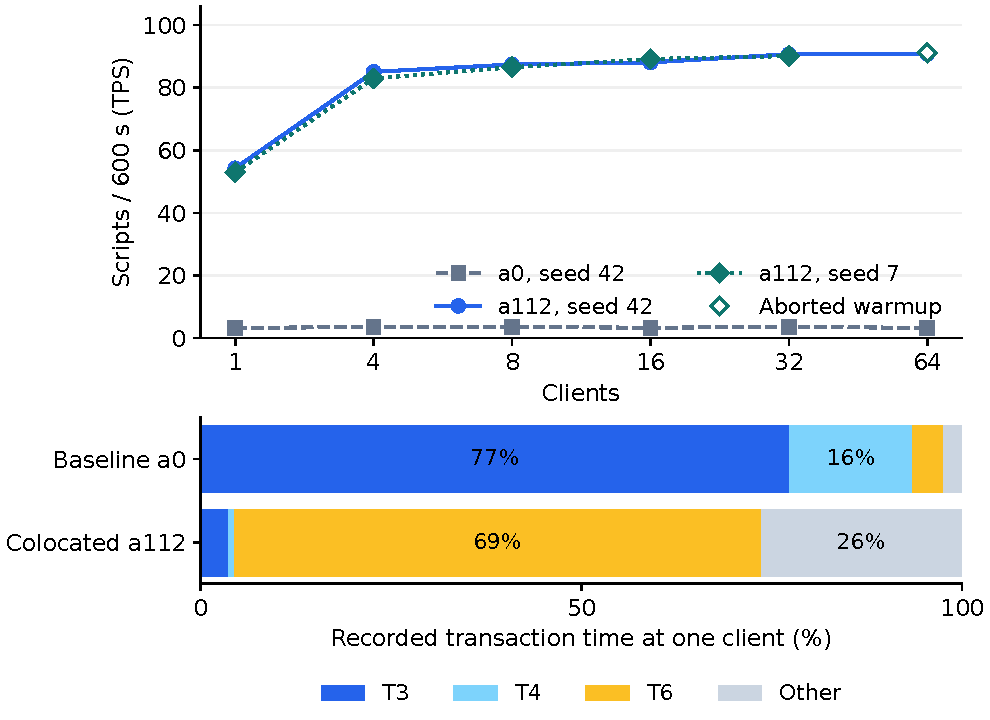
\includegraphics[width=\linewidth]{images/workload-a-full-matched.pdf}
\caption{Matched a0/a112 throughput and recorded transaction-time shares.
The open diamond flags the seed-7 repeat's aborted 64-client warmup.}
\label{fig:a-matched}
\end{figure}

The bottleneck shifted: T6 accounted for approximately 67--83\% of a112's
recorded transaction time, and throughput levelled off around 85--91 TPS from
four clients onward. More concurrency increased latency without proportional
throughput gains.

A seed-7 repeat, job 978177, produced measured TPS within 2.5\% of the seed-42
observations. Its 64-client warmup aborted, excluding that case from comparisons
requiring both phases to complete. Worker serialization cancellation was
reported as a Citus shard-commit error, which pgbench did not retry. The
repeat supports the observed performance while exposing an unresolved
concurrency limitation.
\evidence{\expt{a0}/job 977740; \expt{a112}/jobs 977773 and 978177.
Tables use \code{summary.csv}; the figure also uses \code{transaction_metrics.csv}.
Warmup and measurement exits were checked against the phase logs.}

% Hikaru.
\subsection{\expt{a114}: Maintained sales summaries}
After T6 became dominant, a114 added exact daily sales summaries to a112.
The summaries were maintained synchronously, with eight stripes per merchant/day
to spread updates. The motivation was to reduce repeated aggregation of raw
orders, following the general pre-aggregation approach in Citus's analytics
documentation \citep{citus-realtime}.

In the scale-1, four-client diagnostic, job 979865 achieved 85.333 TPS versus
92.383 TPS in the earlier a112 diagnostic. T6's mean latency increased from
650.6 to 764.5\,ms. Core integrity and summary-equivalence checks passed.

The experiment did not demonstrate a benefit. Summaries reduce raw data
aggregation but introduce maintenance and query-execution work. A single
diagnostic does not isolate each cost, but provides no basis for selecting a114.

% Hikaru. This is follow-up evidence, not the final design.
\subsection{\expt{a115}: Timestamp index for T6}
A115 added an index on \code{orders(created_at)} to a112 while retaining the
original T6 query. The four-client diagnostic, job 979866, achieved 288.633 TPS,
with T6's mean reduced to 115.9\,ms. It recorded two retry attempts, no failed
measured transactions and passing validation. We then ran full seed-42 and
seed-7 experiments.

\begin{table}[htbp]
\caption{A115 full-run outcomes. TPS is shown only if both phases completed.}
\label{tab:a115}
\begin{tabularx}{\linewidth}{@{}rYY@{}}
\toprule
\textbf{Clients} & \textbf{Seed 42: job 979909} & \textbf{Seed 7: job 979910} \\
\midrule
1 & 115.485 TPS; zero failures & 109.893 TPS; zero failures \\
4 & 296.697 TPS; one serial. failure & 276.233 TPS; zero failures \\
8 & 335.585 TPS; zero failures & Measurement aborted \\
16 & 323.213 TPS; zero failures & Measurement aborted \\
32 & Measurement aborted & 330.600 TPS; zero failures \\
64 & Warmup and measurement aborted & Warmup and measurement aborted \\
\bottomrule
\end{tabularx}
\end{table}

Seven of twelve cases completed both phases; six also had zero failed records.
All twelve post-run integrity checks passed, but that does not make aborted
performance measurements suitable for ranking.

The aborts share one failure mode. In 17 of the 19 client aborts across both
seeds, pgbench stopped at T1's \texttt{COMMIT} with a Citus ``could not commit
transaction for shard'' error; the other two occurred in T2 and T9. In these logs, worker
serialization cancellations surfaced as shard-commit errors that pgbench did
not retry. Commit failures limited reliable high-concurrency results; the runs
do not independently isolate their cause.

At one client, a115 achieved $2.13\times$ and $2.07\times$ the throughput of the
corresponding a112 seeds. The index has promising measured benefits, but neither
seed produced a complete successful matrix. We retained a115 as follow-up
evidence and selected a112 as the final A design.
\evidence{\expt{a115}, jobs 979866, 979909 and 979910; full-run outcomes were
checked against warmup/measurement exits, raw logs and validation records.}

% Kelvin.
\subsection{\expt{a10}: Autocommit for single-statement updates}
\label{sec:a10}
Kelvin's write-path experiments start from a102. On that base, T3 and T4
still dominate recorded time, limiting the effect of faster updates on TPS.
The full experiments retain scale 1, the workload mix, SERIALIZABLE isolation,
60-second warmups and 600-second measurements.

A10 removes explicit BEGIN and COMMIT commands around T2, T5, T8 and T9.
Each already consists of one UPDATE, including T2's stock-validity predicate.
Autocommit removes separate transaction-control commands while retaining
statement atomicity and the configured isolation level.

\begin{table}[htbp]
\caption{Median latency, a102 $\rightarrow$ a10, in milliseconds.}
\label{tab:a10}
\begin{tabularx}{\linewidth}{@{}lZZZZ@{}}
\toprule
\textbf{Txn} & \textbf{1 client} & \textbf{4 clients} &
\textbf{8 clients} & \textbf{64 clients} \\
\midrule
T2 & $1.543 \to 1.053$ & $2.427 \to 1.549$ & $6.035 \to 2.728$ & $11.742 \to 6.730$ \\
T5 & $1.377 \to 0.920$ & $2.180 \to 1.204$ & $5.585 \to 1.431$ & $11.954 \to 6.708$ \\
T8 & $1.678 \to 1.145$ & $2.285 \to 1.414$ & $5.331 \to 1.742$ & $15.167 \to 9.183$ \\
T9 & $1.460 \to 1.039$ & $2.766 \to 1.243$ & $7.285 \to 3.733$ & $13.463 \to 5.896$ \\
\bottomrule
\end{tabularx}
\end{table}

Median latency decreased by approximately 29--74\% across these sixteen
comparisons, and p95 improved in twelve. Low transaction counts make T8/T9 tail
estimates less stable. The 16-client comparison is excluded because a102's
warmup aborted; the 32-client comparison is excluded because a10's measurement
aborted during unchanged T1.

The consistent median improvements support reducing transaction-control round
trips. Overall TPS did not improve consistently because expensive reads remained
unchanged. We retain a10 separately: it was not benchmarked on top of a112
and is not part of the measured final design.
\evidence{\expt{a102}/job 965657 and \expt{a10}/job 966308,
\code{transaction_metrics.csv} and phase logs.}

% Kelvin. This is also the control for a11.
\subsection{\expt{a14}: Maintenance before benchmarking}
Experiment a14 runs \texttt{VACUUM (ANALYZE)} on each table after loading, followed by
\texttt{CHECKPOINT} on all five nodes. The motivation was to reduce interference
from dead tuples and pending writes left by data generation. It also provides
the maintenance control for a11.

Job 967194 showed no consistent overall TPS or transaction-latency benefit.
At eight clients, T9's median decreased but T8's increased. One final
serialization failure occurred at 32 clients. The experiment did not justify
including this procedure in the final A design; its principal value was as
a control for fillfactor.
\evidence{\expt{a14}/job 967194: \code{hot_updates.csv},
\code{transaction_metrics.csv} and \code{summary.csv}.}
% Kelvin. Compare to a14 to isolate fillfactor.
\subsection{\expt{a11}: Fillfactor and HOT updates}
A11 retains a14's maintenance and sets \code{fillfactor = 80} on customers,
products, inventory and orders. Leaving free space can enable heap-only tuple
(HOT) updates when the relevant indexed columns are unchanged, avoiding new
entries in ordinary indexes \citep{pg-hot}. Kelvin collected update statistics
from worker shards before and after each measured run, outside the timed interval.

\begin{table}[htbp]
\caption{HOT share of updates across six client counts.}
\label{tab:a11}
\begin{tabularx}{\linewidth}{@{}YZZ@{}}
\toprule
\textbf{Table} & \textbf{a14: default fillfactor} & \textbf{a11: fillfactor 80} \\
\midrule
Inventory & 23.3--37.0\% & 100\% \\
Orders & 76.2--81.5\% & 100\% \\
Customers & 0--19.0\% & 100\% \\
Products & 1.8--12.8\% & 100\% \\
\bottomrule
\end{tabularx}
\end{table}

All recorded a11 updates were HOT and none moved to a new page. Nevertheless,
overall TPS and write latency did not improve consistently. Inventory received
only about 2,500--3,100 updates per ten-minute measurement across four workers,
because distributed reads still limited throughput. Avoiding index maintenance
at that rate had limited effect on total runtime.

Lower fillfactor also has a storage trade-off. T6's one-client median increased
from 266.425 to 280.749\,ms, consistent with a larger footprint, though this
experiment does not independently establish the cause. A11 recorded zero retries
at every client count; repetition is needed before attributing that observation
to fillfactor. Testing the change on a112 remains future work.
\evidence{\expt{a14}/job 967194 and \expt{a11}/job 967195:
\code{hot_updates.csv}, \code{transaction_metrics.csv} and \code{summary.csv}.}

% Kelvin. Do not claim synchronous_commit=off disables two-phase durability.
\subsection{\expt{a12}: Asynchronous commit}
A12 sets \code{synchronous_commit = off} on the coordinator and workers to
investigate WAL-flush waiting. Asynchronous commit can acknowledge ordinary
transactions before their WAL is durable, risking loss of recently acknowledged
transactions after a crash. PostgreSQL specifies that two-phase-commit commands
remain synchronous, so the setting does not remove every durability wait from
distributed transactions \citep{pg-async}.

Job 967217 showed some lower single-row update latencies, but similar changes
occurred in a14 without changing commit behaviour. At eight clients, T2's median
was 4.613\,ms in a12 and 4.759\,ms in a14, compared with 6.035\,ms in a102.
T1's one-client median changed from approximately 11.68 to 11.86\,ms.
These results do not establish WAL-flush waiting as the dominant cost.

A12 provided no convincing overall throughput benefit while weakening durability for affected transactions. We excluded it from the final design.
\evidence{\expt{a12}/job 967217, compared with \expt{a102}/job 965657 and
\expt{a14}/job 967194. An earlier a12 submission, job 967193, was allocated
xcnc nodes and cancelled; it is kept in the archive but not compared.}
% Both A authors. Local-only tests must not be presented as full benchmarks.
\subsection{Supporting experiments, validation and final selection}
An unrun proposal, a13, would have imposed a fixed lock order on T7. We did
not run it because the preserved baseline recorded serialization failures,
not deadlock failures. A deadlock-prevention rewrite would not directly
address that error category \citep{pg-isolation}.

Local-only implementations explored a one-call T1 function, maintained
summaries, memory settings, executor concurrency and alternative read-only
declarations. They supported implementation and correctness testing; their
small datasets and short runs do not substitute for course-cluster benchmarks.
Their code is packaged under \code{supporting_implementations/local_only/},
with outputs under \code{evidence/local-only/}.

Validation covered inventory non-negativity, order totals, identifier uniqueness,
rollback behaviour, placement metadata and selected transaction semantics.
Tests included transfers with different inventory and product identifiers.
Validation ran outside the timed interval. Passing checks establish the tested
invariants at inspected checkpoints, not correctness under every concurrent
schedule. Passing checks after an abort do not make a performance run successful.

\textbf{A112 is the final Workload A design.} It supplies a complete successful
seed-42 matrix and a substantial matched improvement. A115 is a promising but
unreliable follow-up. A10 demonstrates a separate transaction-level improvement
that has not yet been combined with a112.

